\section{Evaluation}
\label{sec:eval}
\subsection{Experimental Setup}
\label{subsec:expsetup}
For this work I implemented two scripts using Python 3.6.5. The two scripts represent the two stages of clustering and classification shown in Figure~\ref{fig:actual}; the first script, named \texttt{clustering.py}, performs the clustering and saves the intermediate representation as a .csv file called \texttt{[appname]\_dataset.csv}. This file is then read as input by \texttt{classifier.py} which will consequently perform the classification using the Random Forest algorithm presented in Section~\ref{subsubsec:rfc}. The computed performance measures will be printed to \texttt{stdout}.

It has to be noted that I trained a model for each different application, this means that the model that classifies Facebook actions has no way to classify Twitter actions since none of the Twitter flows has been shown to it during the clustering process or during the Random Forest training phase.

Most of the actions collected in the initial dataset are deemed to be not privacy-violating by the original authors; I do share their opinion, for this reason, before training the Random Forest, I renamed all the labels of the non relevant actions as \textit{other}. This operation is done in memory by the \texttt{classifier.py} script, in this way the intermediate dataset stays untouched and many different configuration of relevant actions can be tried. The list of relevant action for each app can be found inside \texttt{classification.py}.


\subsubsection{Computational Issues}
Because of some issues with the functions provided by the \textit{SciPy} library, I had to keep in memory the distance matrix of the flows. In the distance matrix $D$ each entry $(i,j)$ contains the value of $dtw(i, j)$ which makes $D$ symmetric; this allows me to reduce by half the memory needed for the matrix since I could just compute the triangular upper (or lower) part of $D$. Unfortunately this ``optimization'' was not enough; the amount of memory needed was way higher that what my Google Cloud machine had. For this reason I decided to reduce the dataset to about 10,000 flows per application; again this is done in memory by the \textit{clustering.py} script, therefore the original dataset is not modified. The number of actions in the initial and intermediate datasets can be seen in Table \ref{tab:datasetdata}.

\begin{table}[!h]
\centering
\begin{tabular}{|l|c|c|c|}
\hline
      & \multicolumn{2}{c|}{Original Dataset} & Intermediate Dataset \\ \hline
         & \textbf{Flows}    & \textbf{Actions [unique labels]}    & \textbf{Actions}              \\ \hline
\textbf{Dropbox}  & 48462    & 15103 [33]                 & 3138                 \\ \hline
\textbf{Evernote} & 17014    & 6214 [32]                  & 4239                 \\ \hline
\textbf{Facebook} & 50319    & 12468 [41]                 & 2494                 \\ \hline
\textbf{GMail}    & 9924     & 5644 [38]                  & 5644                 \\ \hline
\textbf{GPlus}    & 33471    & 17573 [38]                 & 5727                 \\ \hline
% \textbf{Tumblr}   & 56702    & 14989 [47]                 & 2726                 \\ \hline
\textbf{Twitter}  & 36259    & 7334 [25]                  & 2009                 \\ \hline
\end{tabular}
\caption{\small{The table shows the different number of actions for the different datasets. The smaller number of actions in the intermediate datasets is the result of limiting the number of flows to about 10,000 per application.}}
\label{tab:datasetdata}
\end{table}


\subsubsection{Differences from the original work}
Apart from the smaller number of flows used for training phase, there are still other differences from the original work throughout my implementation. First of all the original authors weighted differently incoming and outgoing packets, secondly, they never considered all the packets of a flow, but, through statistical analysis, they decided take into consideration only packets who were to be found in specific hard coded ranges. Both these approaches allowed them to test different configurations which then lead to a maximization of the performance of the classifier. Same thing goes for the number of clusters: they evaluated the fitness of the clustering based on the random forest performances on it, this means that the number of clusters $k$ they chose was obtained through this form of parameter tuning. While I do agree on the methodology they used, I am not able to follow the same path due mainly to time and computational constraints. Luckily, however, by looking at the images of the original work (Figure \ref{fig:original}) I could grasp that the best value for $k$, the number of clusters, was close to 250, which is the value I used for this work.  

\subsection{Experimental Results}
In Table \ref{tab:results} are shown the results using the same metrics employed in the original work: \textit{precision} ($P$), \textit{recall} ($R$), and \textit{F1 measure} ($F_1$). Being this a multiclass problem (the multiple classes being the \textit{action labels}), the shown results are the weighted averages of the measures obtained for each class. The scores are almost identical to those achieved in the original work as shown in Figure~\ref{fig:original}. 

\begin{table}[h]
\centering
\begin{tabular}{l|ccc}
\hline
         & $P$ & $R$ & $F_1$ \\ \hline
Dropbox  & 0.87    &  0.91   &    0.88   \\
Evernote & 0.95   &  0.95   &    0.95   \\
Facebook &  0.99   &  0.99   &  0.98     \\
GMail    &   0.86  &   0.91  &   0.88    \\
GPlus    &  0.78   &  0.81   &   0.79    \\
Twitter  &  0.99   &  0.99   &   0.99    \\ \hline
\end{tabular}
\caption{Precision, recall, and F1 values for the different apps. }
\label{tab:results}
\end{table}

\begin{figure}[h]
\centering
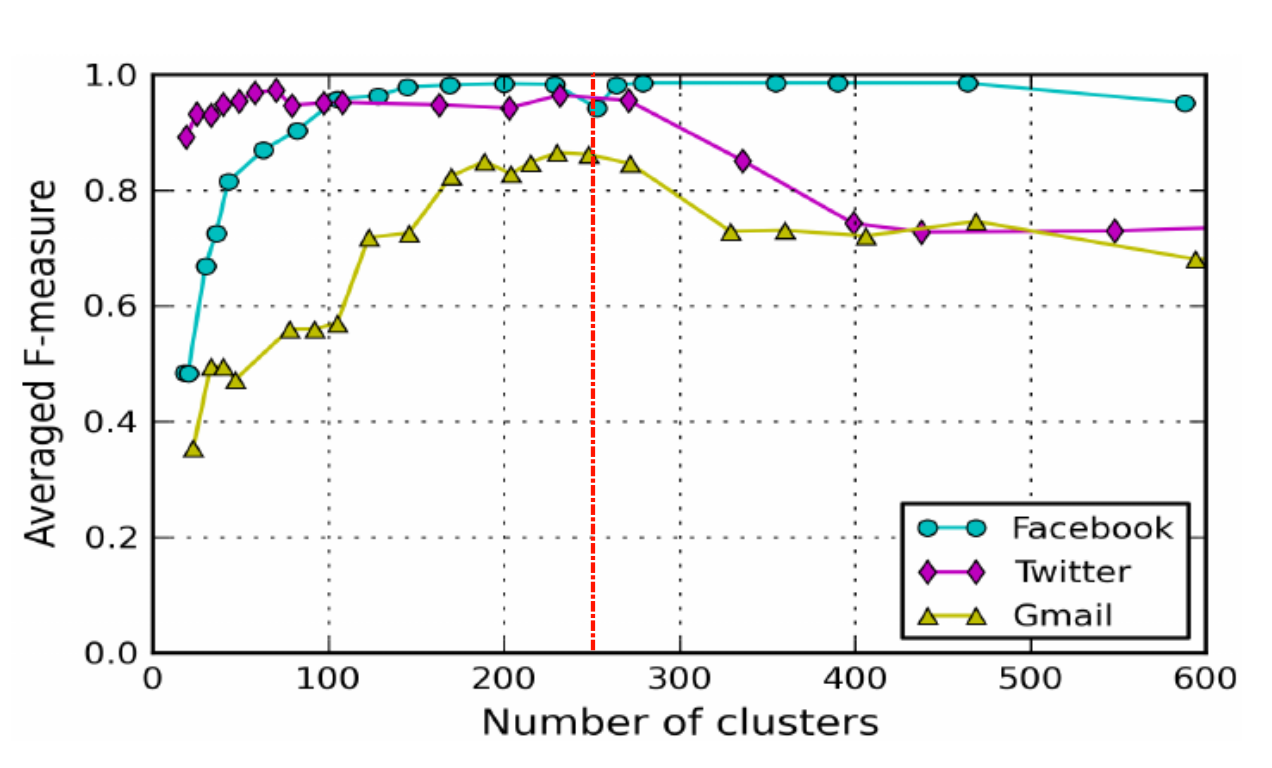
\includegraphics[scale=0.5]{images/fig10}
  \label{fig:sfig1}
\caption{The performances of the classifier used by the original authors for different number of clusters. This figure is taken from \cite{contiknocking} just for comparison; it shows that for $k=250$ (marked by the red vertical line), the original authors and I achieved more or less same performances.}
\label{fig:original}
\end{figure}

% ['dropbox', 'evernote', 'facebook', 'gmail', 'gplus', 'tumblr',
%        'twitter'], dtype=object), array([48462, 17014, 50319,  9924, 33471, 56702, 36259]))

% actions in original dataset
% Actions for dropbox: 15103
% Actions for evernote: 6214
% Actions for facebook: 12468
% Actions for gmail: 5644
% Actions for gplus: 17573
% Actions for tumblr: 14989
% Actions for twitter: 7334

% unique action labels
% Actions for dropbox: 33
% Actions for evernote: 32
% Actions for facebook: 41
% Actions for gmail: 38
% Actions for gplus: 38
% Actions for tumblr: 47
% Actions for twitter: 25

% unique
% Actions for dropbox: 33
% Actions for evernote: 32
% Actions for facebook: 40 <-- one action is not represented in the intermediate dataset
% Actions for gmail: 38
% Actions for gplus: 38
% Actions for tumblr: 47
% Actions for twitter: 25

% actions (rows) in intermediate
% Actions for dropbox: 3138 
% Actions for evernote: 4239
% Actions for facebook: 2494
% Actions for gmail: 5644
% Actions for gplus: 5727
% Actions for tumblr: 2726
% Actions for twitter: 2009

